% -------------- PREAMBULO ------------ %
\documentclass[a4paper, 12pt]{report}
\usepackage[left = 3cm, top = 2.5cm, bottom = 3cm, right = 2.5cm]{geometry}
\usepackage[spanish]{babel}
\usepackage[utf8]{inputenc}  %Uso de simbolos directamente del teclado
\usepackage[T1]{fontenc}     %Salida 
\usepackage{graphicx}        %Manejo de figuras y graficos
\usepackage{booktabs}        %Para formar tablas
\usepackage{color}           %Para usar colores
\usepackage{setspace}        %Usado para doble espacio, espacio y medio y espacio simple (\onehalfspace  \doublespacing  \singlespace)
\usepackage{enumitem}        %Para enumerar
\usepackage{ragged2e}
\usepackage{times}			 %Tipo de letra
\usepackage{anyfontsize}     %PErmite usar modificar los tamaños de letra
\usepackage{titlesec}	     %Modificar el titulo
\setcounter{secnumdepth}{3}  %Para que ponga 1.1.1.1 en subsubsecciones
\setcounter{tocdepth}{3}     %Para que ponga subsubsecciones en el indice
\bibliographystyle{apalike}  %Bibliografía Norma APA

%                            Crear colores                      %     
\definecolor{rosaclaro}{RGB}{247,180,180}

%                            redefiniendo comandos              %
\renewcommand{\chaptername}{\bf{\large{\underline{CAP\'ITULO}}}}
\titleformat{\chapter}[display]{\normalfont}{\bf\large\filcenter\large\ \underline{CAP\'ITULO \thechapter}}{0.5em}{\large\bfseries\filcenter\underline}

% -------------- CUERPO ------------ %
\begin{document}
%%%%%%%%%%%%%%%%%%%%%%%%%%%% PORTADA %%%%%%%%%%%%%%%%%%%%%%%%%%%%
\pagestyle{empty}                          
\spacing{1.2}

\begin{center}
 {\bf {\fontsize{18}{20.8}\selectfont UNIVERSIDAD NACIONAL DE TRUJILLO}}  
  
 {\bf{\fontsize{16}{18.8}\selectfont Facultad de Ciencias Físicas y Matemáticas}} 
 
 {\bf{\fontsize{16}{18.8}\selectfont Escuela Académico Profesional de Informática}} 	
\end{center}  

\vskip .5cm
\begin{figure}[ht]
	\begin{center}
		
\includegraphics[width=.3\textwidth]{unt}
	\end{center}
\end{figure}

\begin{center}
	{\bf {\fontsize{18}{20.4}\selectfont{Monograf\'ia que como parte del curso de T\'opicos en Procesamiento Paralelo:}}}
	
	{\bf {\fontsize{19}{20.4}\selectfont{\vskip .2cm ``Estado del Arte de Cloud Computing''}}}
\end{center}   

\vskip 1.5cm
{\bf {\fontsize{17}{20.4}\selectfont{Nombre de autor(es):}}} 

\begin{center}
	\fontsize{14}{16.8}\selectfont{\'Alvarez Carbajal, Gaby Yuri}		
	
	\fontsize{14}{16.8}\selectfont{Cruz Leyva, Segundo Junior}
	
	\fontsize{14}{16.8}\selectfont{Gonza Llaque, Renato Fabrizzio}
	
	\fontsize{14}{16.8}\selectfont{Guevara Liz\'arraga, Mar\'ia Fernanda}
	
	\fontsize{14}{16.8}\selectfont{Lavado Azabache, Jonatan Esleyter}
\end{center}

{\bf {\fontsize{17}{20.4}\selectfont{Nombre del Asesor:\vskip .5cm}}} 
\begin{center}  
{\fontsize{14}{14}\selectfont{Mg. Mendoza, Edwin}}
\end{center}  

\vskip 3cm
\begin{center}    
	{\bf {\fontsize{14}{16.8}\selectfont Trujillo - La Libertad
	\\ 2017 }}
\end{center} 
\newpage
%%%%%%%%%%%%%%%%%%%%%%%%%%%%%%%%%%%%%%%%%%%%%%%%%%%%%%%%%%%%%%%%%%%%%%%%%%%
\pagestyle{plain}
\doublespacing
\pagenumbering{Roman}
%%%%%%%%%%%%%%%%%%%%%%%%%%%% RESUMEN %%%%%%%%%%%%%%%%%%%%%%%%%%%%
\addcontentsline{toc}{chapter}{Resumen}
\vspace*{6em}
\begin{center}
{\bf{\large{\underline{RESUMEN}}}}
\end{center}
\begin{justify}
Holaque hace como esta muy bien esxop me legr qurbfgs tu vida hace triempo bla bla bla bla bla xd xd xd d
\end{justify}
\newpage
%%%%%%%%%%%%%%%%%%%%%%%%%%%%%%%%%%%%%%%%%%%%%%%%%%%%%%%%%%%%%%%%%%%%%%%%%%%



%%%%%%%%%%%%%%%%%%%%%%%%%%%% INTRODCUCCION %%%%%%%%%%%%%%%%%%%%%%%%%%%%
\addcontentsline{toc}{chapter}{Introducción}
\vspace*{6em}
\begin{center}
{\bf{\large{\underline{INTRODUCCI\'ON}}}}
\end{center}
\begin{justify}
Holaque hace como esta muy bien esxop me legr qurbfgs tu vida hace triempo bla bla bla bla bla xd xd xd d
\end{justify}
\newpage
%%%%%%%%%%%%%%%%%%%%%%%%%%%%%%%%%%%%%%%%%%%%%%%%%%%%%%%%%%%%%%%%%%%%%%%%%%%


\singlespacing
%%%%%%%%%%%%%%%%%%%%%%%%%%%% INDICEs %%%%%%%%%%%%%%%%%%%%%%%%%%%%\\
\renewcommand{\contentsname}{\centering\bf{\large{{\'INDICE GENERAL}}}}
\renewcommand{\listfigurename}{\centering\bf{\large{{LISTA DE TABLAS}}}}
\renewcommand{\listtablename}{\centering\bf{\large{{LISTA DE FIGURAS}}}}

\tableofcontents    % indice de materias
\addcontentsline{toc}{chapter}{\'Indice General}
\listoffigures      % indice de figuras
\addcontentsline{toc}{chapter}{Lista de Figuras}
\listoftables       % indice de tablas
\addcontentsline{toc}{chapter}{Lista de Tablas}

%%%%%%%%%%%%%%%%%%%%%%%%%%%%%%%%%%%%%%%%%%%%%%%%%%%%%%%%%%%%%%%%%%%%%%%%%%%
\doublespacing
%%%%%%%%%%%%%%%%%%%%%%%%%%%% CAPITULOS %%%%%%%%%%%%%%%%%%%%%%%%%%%%
%%%%%%%%%%%%%%%%%%%%%%%%%%%% CAPITULO 1 %%%%%%%%%%%%%%%%%%%%%%%%%%%%
\vspace*{5em}
\chapter{COMPUTACI\'ON CLOUD}
\pagestyle{plain}
\pagenumbering{arabic}
\vspace*{-2em}
\begin{justify}
Holaque hace como esta muy bien esxop me legr qurbfgs tu vida hace triempo bla bla bla bla bla xd xd xd d
\end{justify}
\section{Origen De La Computaci\'on Cloud}
\subsection{Computaci\'on Distribuida}
\subsection{Beneficios Y Limitaciones De La Computaci\'pon Distribuida}
\subsection{Implementaciones}
\begin{enumerate}[label=\alph*)]
    \item{Cl\'uster}
    \item{Grid}
    \item{P2P}
\end{enumerate}
\subsection{Evoluci\'on Hacia La Computaci\'on Cloud}
\section{Concepto De La Computaci\'on Cloud}
\begin{justify}
Una definici\'on para la Computaci\'on Cloud es que puede ser visto como un sistema de computaci\'on distribuido orientado al consumidor. Dicho sistema consiste en una agrupaci\'on de ordenadores virtualizados e interconectados que son suministrados din\'amicamente y presentados como uno o m\'as recursos computacionales unificados.
\end{justify}
\section{Caracter\'isticas De La Computaci\'on Cloud}
\begin{justify}
No es necesario disponer de un equipo potente, tan s\'olo de un aparato con conexi\'on a internet; esto debido a que el dispositivo del usuario no realizar\'ia ning\'un proceso complejo y los ficheros pueden guardarse en la nube. Los servidores en donde se hallan los programas que se utilicen son los encargados de las tareas complicadas que antes se realizaba localmente.
\end{justify}
Algunas caracter\'isticas de la Computaci\'on Cloud, seg\'un \cite{oscarAvilaMejia}, son:
\begin{itemize}
    \item{Escalabilidad:} El sistema establece un nivel de servicios que crea nuevas instancias de acuerdo a la demanda de operaciones existente de tal forma que se reduzca el tiempo de espera y los cuellos de botella.
    \item{Virtualizaci\'on:} Las aplicaciones son independientes del hardware en el que corran. El usuario es libre de usar la plataforma que desee en su terminal (Windows, Unix, Mac, etc.), al utilizar las aplicaciones existentes en la nube puede estar seguro de que su trabajo conservar\'a sus caracter\'isticas bajo otra plataforma.
    \item{Autoreparable:} En caso de surgir un fallo, el \'ultimo respaldo (backup) de la aplicaci\'on se convierte autom\'aticamente en la copia primaria y a partir de \'esta se genera uno nuevo.
    \item{Seguridad:} El sistema permite a diferentes clientes compartir la infraestructura sin preocuparse de comprometer su seguridad y privacidad; de esto se ocupa el sistema proveedor que se encarga de cifrar los datos.
    \item{Disponibilidad:} No se hace necesario guardar los documentos del usuario en su computadora o en medios f\'isicos ya que la informaci\'on radicar\'a en Internet permitiendo su acceso desde cualquier dispositivo conectado a la red.
    \item{Precios:} La computaci\'on cloud no requiere una inversión adicional. No se requiere ning\'un gasto de capital. Los usuarios pagan por servicios y capacidad cuando los necesitan.
\end{itemize}
\section{Clasificaci\'on De Las Soluciones Computaci\'on Cloud}
\subsection{Seg\'un Modelos De Servicio}
\begin{justify}
La computación en nube puede ser vista como una colección de servicios, la cual puede ser presentada como una arquitectura en capas, como se muestra en la figura \ref{fig:capas1}:
\begin{figure}[ht]
	\begin{center}
		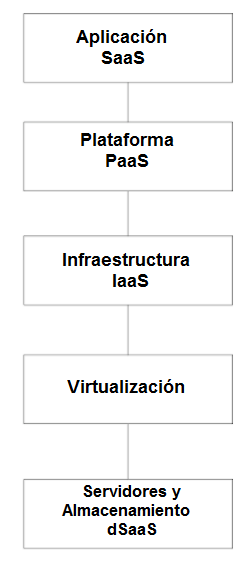
\includegraphics[width=.3\textwidth]{cloudcapas}
		\caption{Arquitectura en capas de computaci\'on cloud \cite{handbook}}
		\label{fig:capas1}
	\end{center}
\end{figure}
\begin{enumerate}[label=\alph*)]
    \item{IaaS:} Se refiere a los recursos informáticos como un servicio. Esto incluye computadoras virtualizadas con potencia de procesamiento garantizada y ancho de banda reservado para almacenamiento y acceso a Internet
    \item{PaaS:} Es similar a IaaS, pero también incluye sistemas operativos y servicios requeridos para una aplicación particular. En otras palabras, PaaS es IaaS con un stack de software personalizado para la aplicación dada.
    \item{SaaS:} Que se muestra en la parte superior de la figura \ref{fig:capas1}. SaaS permite a los usuarios ejecutar aplicaciones de forma remota desde la nube.
    \item{dSaaS:} Proporciona almacenamiento que el consumidor utilizar\'a, incluyendo los requisitos de ancho de banda para el almacenamiento.
\end{enumerate}
\end{justify}

\subsection{Seg\'un Tipo De Nube}
\begin{justify}
Hay tres tipos de computación cloud, los cuales se muestran en la figura \ref{fig:cloudtipos}
\begin{figure}[ht]
	\begin{center}
		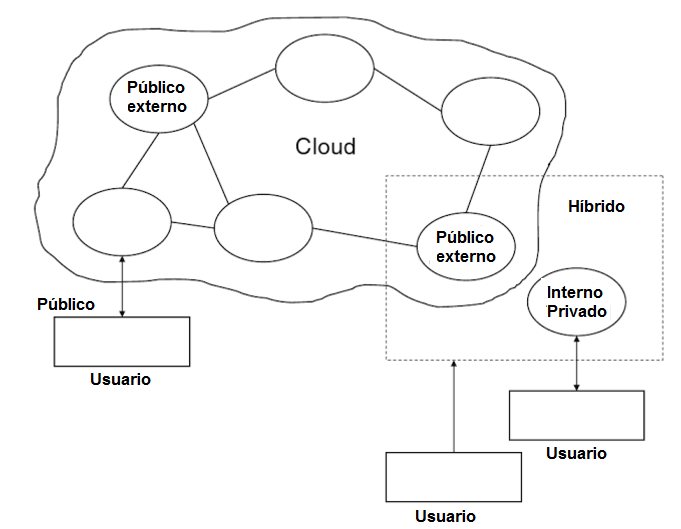
\includegraphics[width=.8\textwidth]{cloudtipos}
		\caption{Tres tipos de computaci\'on cloud \cite{handbook}}
		\label{fig:cloudtipos}
	\end{center}
\end{figure}
\begin{enumerate}[label=\alph*)]
    \item{P\'ublica:} En la nube pública (o en la nube externa), los recursos inform\'aticos se suministran din\'amicamente mendiante Internet a trav\'es de aplicaciones Web o Servicios Web de un proveedor externo (de terceros). Las nubes p\'ublicas son ejecutadas por terceros, y es probable que las aplicaciones de diferentes clientes se mezclen entre sí en los servidores, sistemas de almacenamiento y redes de la nube.
    \item{Privada:} La nube privada (o nube interna) se refiere a la computaci\'on cloud en redes privadas. Las nubes privadas se construyen para el uso exclusivo de un cliente, proporcionando un control total sobre los datos, la seguridad y la calidad del servicio. Las nubes privadas pueden ser construidas y administradas por la propia organización de TI de la empresa o por un proveedor de la nube.
    \item{H\'ibrida:} Un entorno de nube híbrido combina los modelos de nube pública y privada. Las nubes híbridas introducen la complejidad de determinar cómo distribuir aplicaciones a través de una nube pública y privada
    \item{Comunitaria:} El modelo de nube comunitaria permite el acceso a un número de organizaciones o consumidores que pertenecen a una comunidad y el modelo se construye para servir a algún propósito común y específico. Es para el uso de alguna comunidad de personas u organizaciones que comparten preocupaciones comunes en funcionalidades empresariales, requisitos de seguridad, etc. Este modelo permite compartir infraestructura y recursos entre múltiples consumidores pertenecientes a una única comunidad y por lo tanto se hace más barato comparado con una nube privada \cite{sandeep}
\end{enumerate}
\end{justify}

\subsection{Según Por Agentes Intervinientes En El Negocio}
\begin{justify}
Los agentes intervinientes en el negocio seg\'un \cite{tratecno}, se muestran en la figura \ref{fig:agentesintervinientes}
\begin{figure}[ht]
	\begin{center}
		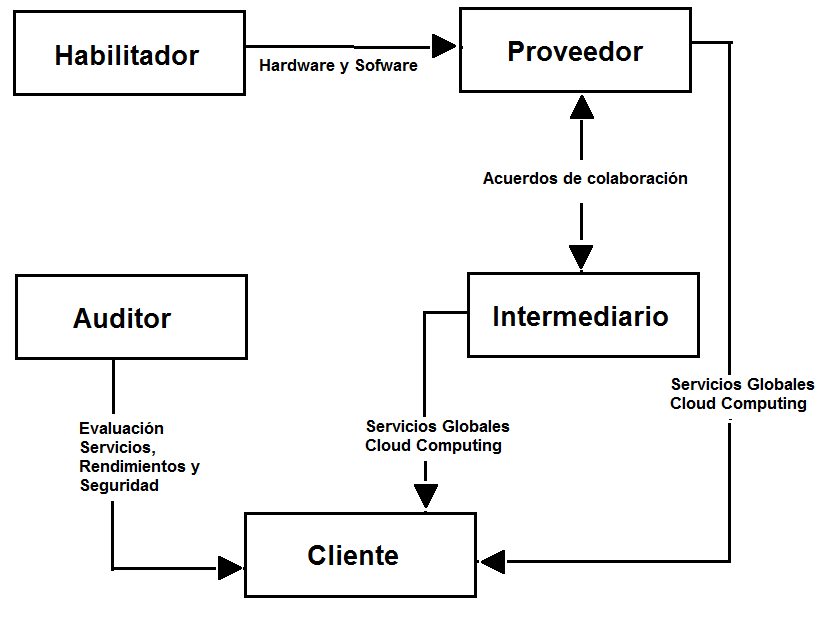
\includegraphics[width=.6\textwidth]{agentesintervinientes}
		\caption{Agentes intervinientes en el negocio \cite{tratecno}}
		\label{fig:agentesintervinientes}
	\end{center}
\end{figure}
\begin{enumerate}[label=\alph*)]
    \item{Habilitador:} Enfocados a ofrecer una serie de servicios Hardware o Software a otros proveedores.
    \item{Proveedor:} Los servicios que presta a los intermediarios y clientes, o bien los genera directamente el, o los contrata a otros proveedores o habilitadores.
    \item{Auditor:} Las funciones a desarrollar por los auditores, son las de llevar a cabo evaluaciones de los servicios, rendimientos y seguridad de las operaciones en el uso de las soluciones Cloud.
    \item{Intermediario:} Los intermediarios adecuan las soluciones para los clientes negociando los distintos servicios, añadiéndole en muchos casos ciertos servicios adicionales como pueden ser algunos apoyos en formación, implementación, etc.
    \item{Cliente:} Dentro del esquema de los agentes intervinientes, es aquel que va a contratar los servicios del resto de los agentes.
\end{enumerate}

\end{justify}

%%%%%%%%%%%%%%%%%%%%%%%%%%%% CAPITULO 2 %%%%%%%%%%%%%%%%%%%%%%%%%%%%
\vspace*{5em}
\chapter{TITULO DEL CAPITULO 2}
\vspace*{-2em}
\begin{justify}
Holaque hace como esta muy bien esxop me legr qurbfgs tu vida hace triempo bla bla bla bla bla xd xd xd d
\end{justify}

%%%%%%%%%%%%%%%%%%%%%%%%%%%% CAPITULO 3 %%%%%%%%%%%%%%%%%%%%%%%%%%%%
\vspace*{5em}
\chapter{TITULO DEL CAPITULO 3}
\vspace*{-2em}
\begin{justify}
Holaque hace como esta muy bien esxop me legr qurbfgs tu vida hace triempo bla bla bla bla bla xd xd xd d
\end{justify}

%%%%%%%%%%%%%%%%%%%%%%%%%%%% CAPITULO 4 %%%%%%%%%%%%%%%%%%%%%%%%%%%%
\vspace*{5em}
\chapter{TITULO DEL CAPITULO 4}
\vspace*{-2em}
\begin{justify}
Holaque hace como esta muy bien esxop me legr qurbfgs tu vida hace triempo bla bla bla bla bla xd xd xd d
\end{justify}

%%%%%%%%%%%%%%%%%%%%%%%%%%%%%%%%%%%%%%%%%%%%%%%%%%%%%%%%%%%%%%%%%%%%%%%%%%%


\newpage
%%%%%%%%%%%%%%%%%%%%%%%%%%%% CONCLUSIONES %%%%%%%%%%%%%%%%%%%%%%%%%%%%
\addcontentsline{toc}{chapter}{Conclusiones}
\vspace*{6em}
\begin{center}
{\bf{\large{\underline{CONCLUSIONES}}}}
\end{center}
\begin{justify}
Podemos concluir muchas cosas v:
\end{justify}
%%%%%%%%%%%%%%%%%%%%%%%%%%%%%%%%%%%%%%%%%%%%%%%%%%%%%%%%%%%%%%%%%%%%%%%%%%%



%%%%%%%%%%%%%%%%%%%%%%%%%%%% BIBLIOGRAFIA %%%%%%%%%%%%%%%%%%%%%%%%%%%%
\addcontentsline{toc}{chapter}{Bibliograf\'ia}
\vspace*{6em}
	\bibliography{Bibliografia}
%%%%%%%%%%%%%%%%%%%%%%%%%%%%%%%%%%%%%%%%%%%%%%%%%%%%%%%%%%%%%%%%%%%%%%%%%%%



\end{document}
